%%%%%%%%%%%%%%%%%%%%%%%%%%%%%%%%%%%%%%%%%
% Formal Text-Rich Title Page 
% LaTeX Template
% Version 1.0 (27/12/12)
%
% This template has been downloaded from:
% http://www.LaTeXTemplates.com
%
% Original author:
% Peter Wilson (herries.press@earthlink.net)
%
% License:
% CC BY-NC-SA 3.0 (http://creativecommons.org/licenses/by-nc-sa/3.0/)
% 
% Instructions for using this template:
% This title page compiles as is. If you wish to include this title page in 
% another document, you will need to copy everything before 
% \begin{document} into the preamble of your document. The title page is
% then included using \titleGP within your document.
%
%%%%%%%%%%%%%%%%%%%%%%%%%%%%%%%%%%%%%%%%%

%----------------------------------------------------------------------------------------
%  PACKAGES AND OTHER DOCUMENT CONFIGURATIONS
%----------------------------------------------------------------------------------------

\documentclass{article}

\newcommand*{\plogo}{\fbox{$\mathcal{PL}$}} % Generic publisher logo
\usepackage{geometry}
\usepackage{url}
\usepackage{multicol}
\usepackage [english]{babel}
\usepackage [autostyle, english = american]{csquotes}
\MakeOuterQuote{"}
\usepackage{float} % Required for tables and figures in the multi-column environment - they need to be placed in specific locations with the [H] (e.g. \begin{table}[H])
%----------------------------------------------------------------------------------------
%	TITLE PAGE
%----------------------------------------------------------------------------------------


\newcommand*{\titleGP}{\begingroup % Create the command for including the title page in the document
\centering % Center all text
\vspace*{\baselineskip} % White space at the top of the page

\rule{\textwidth}{1.6pt}\vspace*{-\baselineskip}\vspace*{2pt} % Thick horizontal line
\rule{\textwidth}{0.4pt}\\[\baselineskip] % Thin horizontal line

{\Huge CONTROL FLU \\[0.4\baselineskip]  
DATA INSIGHTS}\\[0.4\baselineskip] % Title

\rule{\textwidth}{0.4pt}\vspace*{-\baselineskip}\vspace{3.2pt} % Thin horizontal line
\rule{\textwidth}{1.6pt}\\[\baselineskip] % Thick horizontal line

\scshape % Small caps
\Large{Report 2 of 3}  \\[\baselineskip] % Tagline(s) or further description

\begin{Large}
Consent form return and immunization aversion/receptivity:\\ targeting groups for increased uptake \par % Location and year
\end{Large}
\vspace*{2\baselineskip} % Whitespace between location/year and editors

 \\[\baselineskip]
{\large DISEASE CONTROL UNIT\par} % Editor list
{\itshape Joe Brew\par} % Editor affiliation

\vfill % Whitespace between editor names and publisher logo

 \\[0.3\baselineskip] % Publisher logo
{\scshape December 2014} \\[0.3\baselineskip] % Year published
{\large joseph.brew@flhealth.gov}\par % Publisher

\endgroup}

%----------------------------------------------------------------------------------------
%	BLANK DOCUMENT
%----------------------------------------------------------------------------------------

\setlength\columnsep{20pt}
\usepackage{Sweave}
\begin{document} 


\pagestyle{empty} % Removes page numbers

\titleGP % This command includes the title page
\Sconcordance{concordance:targeting.tex:targeting.Rnw:%
1 79 1 1 0 8 1 1 45 35 1 1 75 1 5 5 1 1 32 1 9 10 1 1 66 1 3 4 1 1 32 1 %
4 15 1 1 70 1 3 4 1 1 32 1 4 40 1 1 32 1 1 1 4 30 0 1 2 7 1 1 46 4 1 1 %
29 1 2 2 1 1 4 56 0 1 2 37 1 1 33 1 1 1 4 30 0 1 2 5 1 1 44 8 1 1 22 1 %
2 2 1 1 4 46 0 1 2 4 1 1 40 1 1 1 20 28 1 1 38 1 1 1 4 30 0 1 2 1 1 1 %
45 5 1 1 4 46 0 1 2 58 1}




\newgeometry{margin = 3.5cm}
\section*{Context}
This is the second in a three-part program evaluation of the "Control Flu" program using a combination of Alachua County Public Schools, Florida Shots, Emerging Pathogens Institute, and Census data.  Report 1 dealt with county-wide pediatric immunization rates from 2011-12 to 2013-14.  This report, on the other hand, covers immunization uptake among Alachua's public school students, with a focus on assessing likelihood of consent form return by sociodemographic traits and (so as to assist with program targeting and identification of groups at greatest risk).  The third and final report (January 2015) will cover the program's impact on absenteeism.  

\section*{Summary}
The likelihood of returning a consent form, as well as the likelihood of consenting to immunization, vary by age, race, sex, and school.  Calculating a statistically-adjusted "performance score" for each school can be useful in establishing missed opportunities for immunization, as well as gauging program performance.   \\


\section*{Details}
This report covers three flu seasons (2011-12 through 2013-14).  Though we have program data for the current (2014-15) flu season, we do not yet have complete Florida Shots data or EPI consent form return data for this year.  An update to this report, taking into account the 2014-15 flu season, will be available by March, 2015.  

\tableofcontents



\newgeometry{margin=2cm}
\begin{center}
\section*{Risk factors for non-return of consent form}
\end{center}
\addcontentsline{toc}{section}{Risk factors for non-return of consent form}
\begin{multicols}{2}

\setkeys{Gin}{width=0.51\textwidth}


%%%%%%%%%%%%%%%%%%%%%%%%%%%%%%%%%%%%%%%%%%%%%%
% GRADE
%%%%%%%%%%%%%%%%%%%%%%%%%%%%%%%%%%%%%%%%%%%%%%

\subsection*{Grade}
\addcontentsline{toc}{subsection}{Grade}

A student's grade is a signficiant predictor of that student's likelihood of both consent form return and immunization.  The direction of this relationship is complex: students' consent form return and immunization rates remain largely constant through elementary school before beginning a sharp decline through middle and high school.  Of note, an elementary schooler is 2.5-3 times more likely than a high-schooler to return a consent form, and approximately 3 times as likely to get immunized (all locations).  

\begin{center}
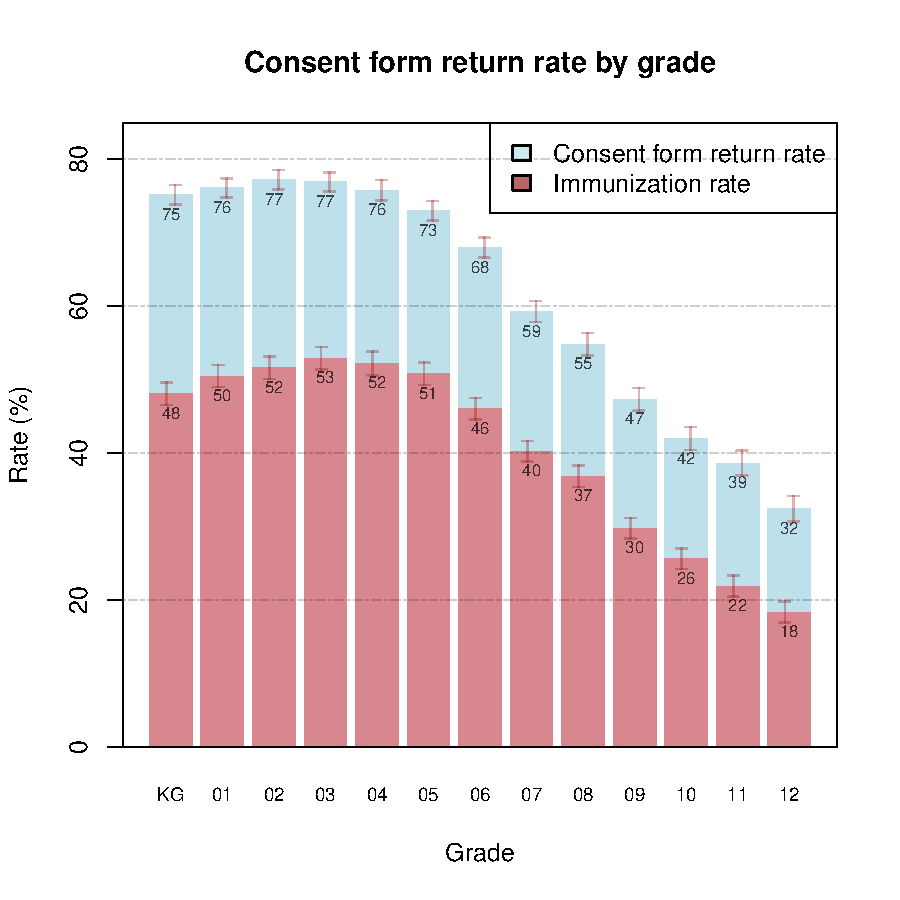
\includegraphics{targeting-002}
\end{center}

Even among those that return a consent form, older students are less likely than their younger counterparts to consent to immunization.  That said, a majority of high-schoolers who return a consent form still want to be immunized.  In other words, \textbf{the drop in immunization in older age groups is primarily due to declining consent form return, not declining immunization receptivity.}   This suggests that interventions aimed at older age groups should focus first and foremost on consent form return (and secondarily on the benefits of immunization).


\begin{center}
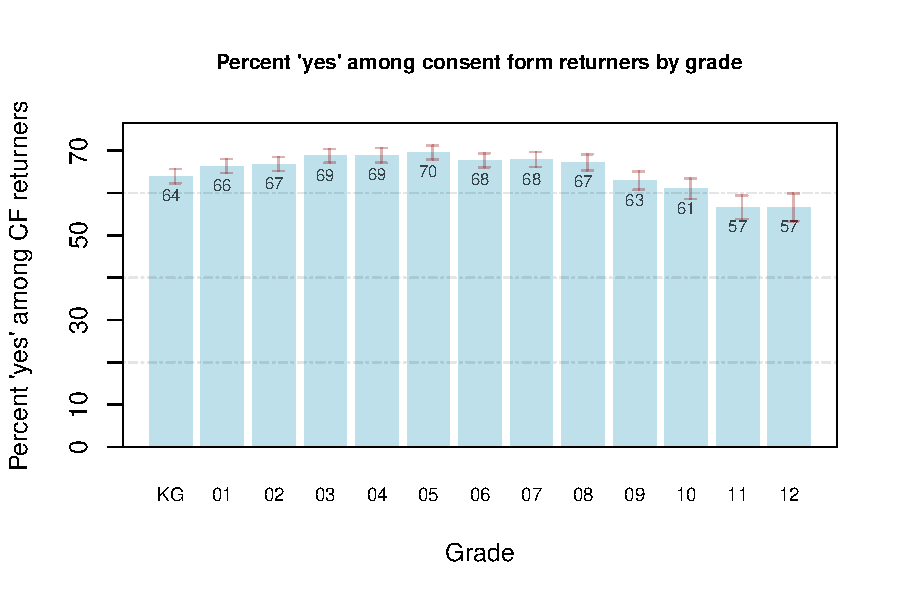
\includegraphics{targeting-003}
\end{center}

%%%%%%%%%%%%%%%%%%%%%%%%%%%%%%%%%%%%%%%%%%%%%%
% RACE
%%%%%%%%%%%%%%%%%%%%%%%%%%%%%%%%%%%%%%%%%%%%%%
\subsection*{Race}
\addcontentsline{toc}{subsection}{Race}

Like age, a student's race is also a significant predictor of consent form return and immunization.  More than three quarters of students of Asian origin return a consent form, whereas fewer than half of African-American students do.  

\begin{center}
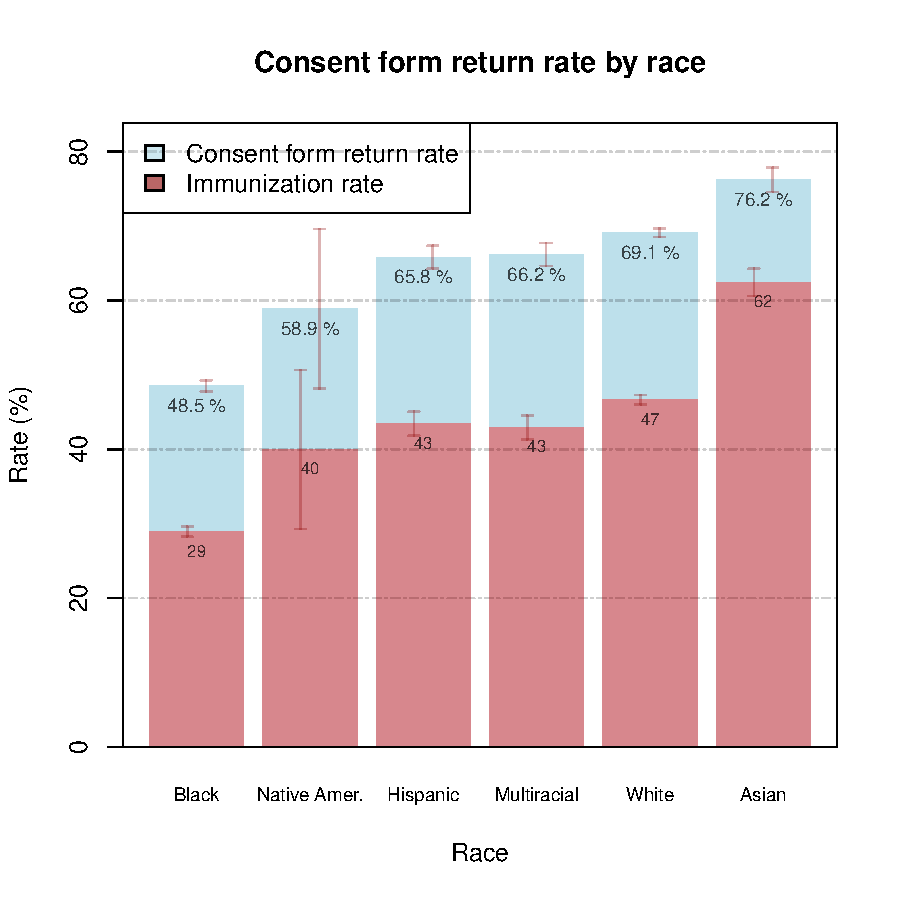
\includegraphics{targeting-004}
\end{center}

Groups with the lowest immunization rates are \emph{not} necessarily adverse to immunization.  On the contrary, among consent form returners, students who are Black, Hispanic or Multiracial have very similar rates of "yes" as their white counterparts.  In other words, \textbf{consent form non-return / loss (not vaccine aversion) explains most of the difference in immunization rates between races.}\footnote{The exception to this is students of Asian origin, who achieve both the highest consent form return rate, as well as the highest percentage of "yes" among consent form returners.  Qualitative research (focus groups or surveys) may be useful in assessing what factors motivate Asian families to be so receptive to vaccination, as findings could help guide interventions for students of other races.}

\begin{center}
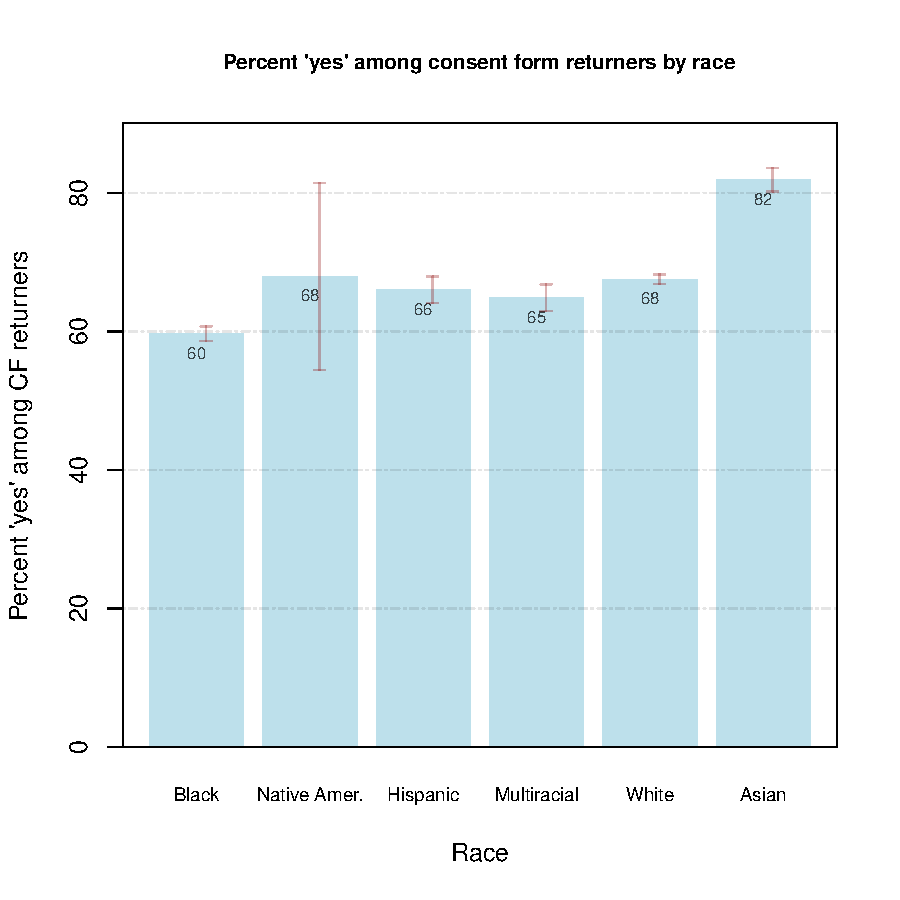
\includegraphics{targeting-005}
\end{center}

The data suggest that non-Asian minority students would have similar levels of immunization as White students \emph{if} similar levels of consent form return could be achieved.  In other words, Black students are nearly as likely to say "yes" to immunization as White students, but far less likely to return a consent form.   Given this reality, efforts at raising immunization rates among minority students should focus on consent form return (rather than education regarding vaccination's benefits). 

\vfill
\columnbreak

%%%%%%%%%%%%%%%%%%%%%%%%%%%%%%%%%%%%%%%%%%%%%%
% SOCIOECONOMIC STATUS
%%%%%%%%%%%%%%%%%%%%%%%%%%%%%%%%%%%%%%%%%%%%%%
\subsection*{Socioeconomic status}
\addcontentsline{toc}{subsection}{Socioeconomic status}
Students who qualify for free/reduced lunch are far less likely to return a consent form than their counterparts.


\begin{center}
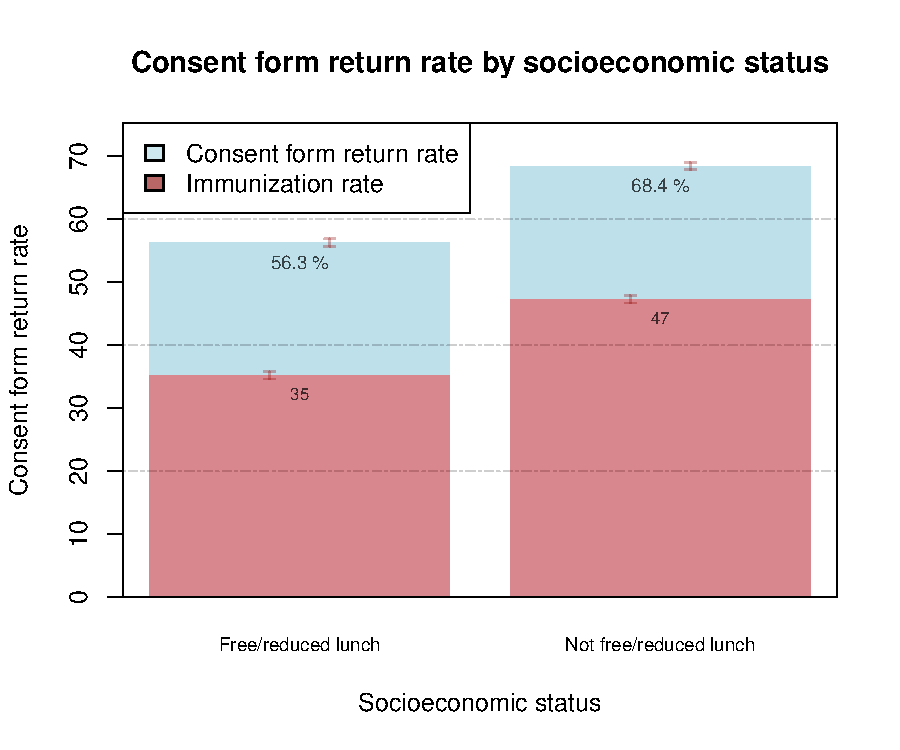
\includegraphics{targeting-006}
\end{center}

That said, when they \emph{do} return a consent form, students on free/reduced lunch are only \emph{slightly} less likely to consent to vaccination than their peers.  

\begin{center}
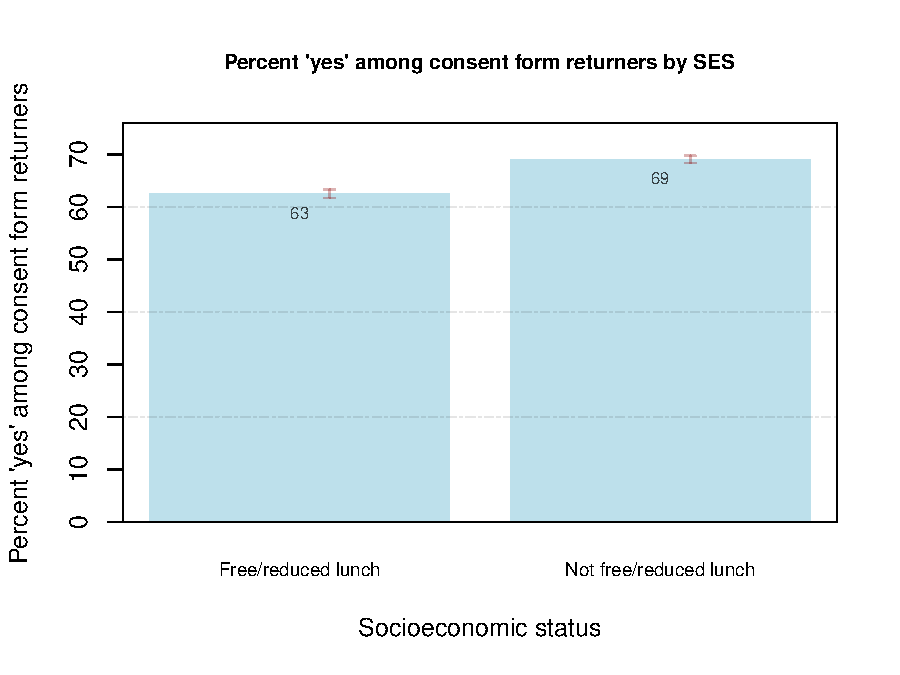
\includegraphics{targeting-007}
\end{center}

In Alachua County, socioeconomic status is largely confounded with race. Students of Asian origin are less likely than white students to qualify for free/reduced lunch, whereas students of all other races/ethnicities are more likely than their white students to qualify. That said, even after statistical "adjustment" for race and socioeconomic status, being Black, Hispanic or on free/reduced lunch are \emph{independent} risk factors for non-immunization and consent form non-return (more on statistical adjustment in the next section).


%%%%%%%%%%%%%%%%%%%%%%%%%%%%%%%%%%%%%%%%%%%%%%
% SCHOOL IMMUNIZATION
%%%%%%%%%%%%%%%%%%%%%%%%%%%%%%%%%%%%%%%%%%%%%%
\newgeometry{margin = 2cm}
\end{multicols}
\begin{center}
\section*{2013-14 school evaluation: immunization}
\end{center}
\addcontentsline{toc}{section}{2013-14 school evaluation: immunization}
\begin{multicols}{2}

\setkeys{Gin}{width=0.49\textwidth}

\subsection*{Summary}
\addcontentsline{toc}{subsection}{Summary}
By calculating an "immunization performance score" which takes into account a school's racial, socioeconomic and age make-up, we can get a better idea of Control Flu program performance at the school level. \\



A direct comparison of schools' immunization and consent form return rates would be inappropriate given schools' different sociodemographic make-ups, especially in light of the differences found in the previous section.  Rather than a "direct" comparison, we can use multivariate modeling to compare a school's "expected" vs. "observed" consent form return rate (CFRR) and immunization rate (IR).  Schools whose observed (real) values differ significantly from their "expected" rates (given their sociodemographic make-up) can be considered to be under- or over-achieving.  \\

\subsection*{Risk factors for non-immunization}
\addcontentsline{toc}{subsection}{Risk factors for non-immunization}


For a first pass, we will construct a multivariate logistic regression model to assess a student's likelihood of immunization, given their race, free/reduced lunch status and age, using only data from the 2011-12 and 2012-13 school years.  The following table shows the results of this model, converted to odds ratios, with the "baseline" group being white, kindergarten-aged, non-free lunch students. \\ 


The "odds ratio" can be interpreted as the likelihood of \emph{not} getting immunized, relative to the baseline group.  Here are two examples of interpretation of the  table :\begin{enumerate}
\item "Holding constant other factors (grade and socioeconomic status), black students are 1.55 more likely than white students to \textbf{not} get immunized against influenza."
\item "After adjustment for other factors (race and socioeconomic status), 12th graders are 4.83 times more likely to \textbf{not} return a consent form than their kindergarten counterparts."
\end{enumerate}

\vfill
\columnbreak


\begin{table}[H]
% latex table generated in R 3.1.1 by xtable 1.7-4 package
% Tue Dec 16 15:47:02 2014
\begin{table}[ht]
\centering
{\small
\begin{tabular}{lrr}
  \hline
Factor & Odds ratio & P-value \\ 
  \hline
Asian & 0.56 & 0.00 \\ 
  Hispanic & 1.37 & 0.00 \\ 
  Black & 1.55 & 0.00 \\ 
  Multiracial & 1.12 & 0.00 \\ 
  Native Amer. & 1.53 & 0.04 \\ 
  Grade 01 & 0.89 & 0.01 \\ 
  Grade 02 & 0.85 & 0.00 \\ 
  Grade 03 & 0.87 & 0.00 \\ 
  Grade 04 & 0.93 & 0.13 \\ 
  Grade 05 & 1.04 & 0.44 \\ 
  Grade 06 & 1.24 & 0.00 \\ 
  Grade 07 & 1.55 & 0.00 \\ 
  Grade 08 & 1.79 & 0.00 \\ 
  Grade 09 & 2.40 & 0.00 \\ 
  Grade 10 & 3.12 & 0.00 \\ 
  Grade 11 & 3.90 & 0.00 \\ 
  Grade 12 & 4.83 & 0.00 \\ 
  Free lunch & 1.55 & 0.00 \\ 
   \hline
\end{tabular}
}
\caption{Factors for immunization} 
\end{table}\end{table}


Having established risk factors for non-immunization at the \emph{student-}level, we can procede to calculate "expected" immunization rates at the school level.  The table on the following page breaks down each school's 2013-14 immunization numbers; the product of a school's "observed" and "expected" rates yields a performance score.  Schools with greater than 1 performed better than expected, whereas schools with lower than 1 performed worse than expected in terms of total immunized students.  \\

When reading the following table, keep in mind that (a) these data \emph{include} vaccinations administered by private practitioners and (b) numbers may differ slightly from previous immunization rate tables, since many data points were excluded from analysis due to quality and compatability issues.\footnote{"Fuzzy" matching algorithms were written specifically for the purpose of matching students from ACPS' database to Florida Shots data, but variations in spelling and mistakes make this task imperfect at best.}



\newgeometry{margin=3cm}
\end{multicols}
\setkeys{Gin}{width=\textwidth}

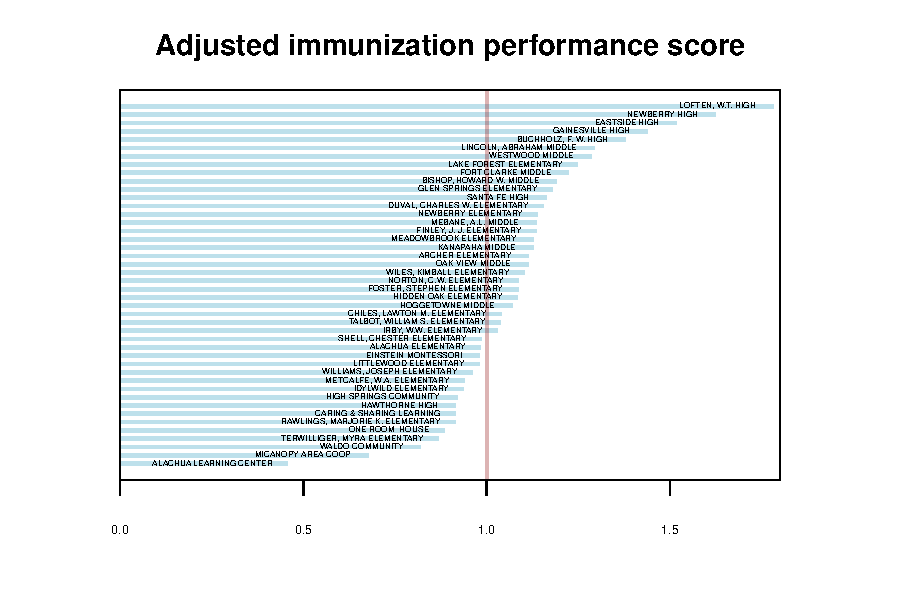
\includegraphics{targeting-011}


\begin{table}[H]
% latex table generated in R 3.1.1 by xtable 1.7-4 package
% Tue Dec 16 15:47:02 2014
\begin{table}[ht]
\centering
{\tiny
\begin{tabular}{lrrrr}
  \hline
SCHOOL & STUDENTS & EXPECTED & OBSERVED & SCORE \\ 
  \hline
LOFTEN, W.T. HIGH  & 207 & 43.23 &  77 & 1.78 \\ 
  NEWBERRY HIGH  & 526 & 122.55 & 199 & 1.62 \\ 
  EASTSIDE HIGH  & 1304 & 289.87 & 440 & 1.52 \\ 
  GAINESVILLE HIGH  & 1802 & 408.08 & 587 & 1.44 \\ 
  BUCHHOLZ, F. W. HIGH  & 2112 & 538.14 & 742 & 1.38 \\ 
  LINCOLN, ABRAHAM MIDDLE  & 662 & 253.55 & 328 & 1.29 \\ 
  WESTWOOD MIDDLE  & 990 & 368.01 & 473 & 1.29 \\ 
  LAKE FOREST ELEMENTARY & 301 & 116.15 & 145 & 1.25 \\ 
  FORT CLARKE MIDDLE  & 875 & 343.90 & 421 & 1.22 \\ 
  BISHOP, HOWARD W. MIDDLE  & 731 & 265.48 & 316 & 1.19 \\ 
  GLEN SPRINGS ELEMENTARY & 493 & 252.63 & 298 & 1.18 \\ 
  SANTA FE HIGH  & 1003 & 246.54 & 287 & 1.16 \\ 
  DUVAL, CHARLES W. ELEMENTARY & 320 & 122.93 & 142 & 1.16 \\ 
  NEWBERRY ELEMENTARY & 498 & 255.44 & 291 & 1.14 \\ 
  MEBANE, A.L. MIDDLE  & 388 & 141.79 & 161 & 1.14 \\ 
  FINLEY, J. J. ELEMENTARY & 576 & 288.94 & 328 & 1.14 \\ 
  MEADOWBROOK ELEMENTARY  & 673 & 354.40 & 400 & 1.13 \\ 
  KANAPAHA MIDDLE  & 974 & 380.58 & 429 & 1.13 \\ 
  ARCHER ELEMENTARY  & 468 & 232.51 & 259 & 1.11 \\ 
  OAK VIEW MIDDLE  & 714 & 295.42 & 329 & 1.11 \\ 
  WILES, KIMBALL ELEMENTARY & 788 & 424.58 & 468 & 1.10 \\ 
  NORTON, C.W. ELEMENTARY & 650 & 321.14 & 349 & 1.09 \\ 
  FOSTER, STEPHEN ELEMENTARY & 473 & 229.38 & 249 & 1.09 \\ 
  HIDDEN OAK ELEMENTARY & 730 & 398.64 & 432 & 1.08 \\ 
  HOGGETOWNE MIDDLE  & 109 & 36.46 &  39 & 1.07 \\ 
  CHILES, LAWTON M. ELEMENTARY & 691 & 360.65 & 375 & 1.04 \\ 
  TALBOT, WILLIAM S. ELEMENTARY & 668 & 362.39 & 376 & 1.04 \\ 
  IRBY, W.W. ELEMENTARY & 427 & 209.86 & 216 & 1.03 \\ 
  SHELL, CHESTER ELEMENTARY & 196 & 90.23 &  89 & 0.99 \\ 
  ALACHUA ELEMENTARY & 370 & 175.78 & 173 & 0.98 \\ 
  EINSTEIN MONTESSORI  & 104 & 46.86 &  46 & 0.98 \\ 
  LITTLEWOOD ELEMENTARY & 584 & 280.61 & 275 & 0.98 \\ 
  WILLIAMS, JOSEPH ELEMENTARY & 540 & 236.33 & 227 & 0.96 \\ 
  METCALFE, W.A. ELEMENTARY & 303 & 120.37 & 113 & 0.94 \\ 
  IDYLWILD ELEMENTARY & 636 & 280.36 & 263 & 0.94 \\ 
  HIGH SPRINGS COMMUNITY  & 885 & 428.25 & 394 & 0.92 \\ 
  HAWTHORNE HIGH  & 291 & 76.43 &  70 & 0.92 \\ 
  CARING \& SHARING LEARNING & 136 & 51.33 &  47 & 0.92 \\ 
  RAWLINGS, MARJORIE K. ELEMENTARY & 299 & 114.80 & 105 & 0.91 \\ 
  ONE ROOM  HOUSE & 184 & 83.72 &  74 & 0.88 \\ 
  TERWILLIGER, MYRA ELEMENTARY & 564 & 244.16 & 212 & 0.87 \\ 
  WALDO COMMUNITY  & 192 & 88.93 &  73 & 0.82 \\ 
  MICANOPY AREA COOP  & 124 & 63.53 &  43 & 0.68 \\ 
  ALACHUA LEARNING CENTER & 105 & 52.48 &  24 & 0.46 \\ 
   \hline
\end{tabular}
}
\caption{Sociodemographic-adjusted immunization performance scores by school} 
\end{table}\end{table}



\newgeometry{margin=2cm}
\begin{multicols}{2}
\setkeys{Gin}{width=0.51\textwidth}

%%%%%%%%%%%%%%%%%%%%%%%%%%%%%%%%%%%%%%%%%%%%%%
% SCHOOL CONSENT FORM RETURN
%%%%%%%%%%%%%%%%%%%%%%%%%%%%%%%%%%%%%%%%%%%%%%
\newgeometry{margin = 2cm}
\end{multicols}
\begin{center}
\section*{2013-14 school evaluation: consent form return}
\end{center}
\addcontentsline{toc}{section}{2013-14 school evaluation: consent form return}
\begin{multicols}{2}

\setkeys{Gin}{width=0.49\textwidth}

\subsection*{Summary}
\addcontentsline{toc}{subsection}{Summary}
As a complement to the "immunization performance score", we can calculate a "consent form performance score" which adjusts for each school's racial, socioeconomic and age make-up.  This score can give an idea of where we are missing opportunities (ie, the socioeconomic and demographic of a student body suggest high consent form return, but performance was low). \\


\subsection*{Risk factors for consent form loss}
\addcontentsline{toc}{subsection}{Risk factors for consent form loss}

The previous two pages outlined program performance using immunization rate as the outcome measure.  Though helpful, immunization rates (adjusted or raw) are not, by themselves, ideal for evaluating program efforts.  Given that vaccination aversion is largely outside of the school (ie, a family may be philosophically opposed to all vaccines), an alternative indicator of program performance at the school level would be \emph{consent form return rate}. \\

Modeling on 2011-12 and 2012-13 data, we can estimate the adjusted odds for consent form return.  These can be interpreted as the likelihood of \emph{not} returning a consent form, relative to the baseline group (again, "baseline" consists of students who are white, not on free/reduced lunch, and of kindergarten age). \\


Here are two specific examples of how the odds ratios to the upper right can be interpreted :\begin{enumerate}
\item "Holding constant other factors (grade and socioeconomic status), black students are 2.22 more likely than white students to  \textbf{not} return a consent form."
\item "After adjustment for other factors (race and grade), students who qualify for free lunch are 1.57 times more likely to \textbf{not} return a consent form than their non-free lunch counterparts."


\begin{table}[H]
% latex table generated in R 3.1.1 by xtable 1.7-4 package
% Tue Dec 16 15:47:03 2014
\begin{table}[ht]
\centering
{\small
\begin{tabular}{lrr}
  \hline
Factor & Odds ratio & P-value \\ 
  \hline
Asian & 0.68 & 0.00 \\ 
  Hispanic & 1.09 & 0.10 \\ 
  Black & 2.22 & 0.00 \\ 
  Multiracial & 1.23 & 0.00 \\ 
  Native Amer. & 1.48 & 0.18 \\ 
  Grade 01 & 0.91 & 0.14 \\ 
  Grade 02 & 0.90 & 0.10 \\ 
  Grade 03 & 0.93 & 0.27 \\ 
  Grade 04 & 1.01 & 0.84 \\ 
  Grade 05 & 1.06 & 0.35 \\ 
  Grade 06 & 1.57 & 0.00 \\ 
  Grade 07 & 2.64 & 0.00 \\ 
  Grade 08 & 3.41 & 0.00 \\ 
  Grade 09 & 4.05 & 0.00 \\ 
  Grade 10 & 5.14 & 0.00 \\ 
  Grade 11 & 6.13 & 0.00 \\ 
  Grade 12 & 9.08 & 0.00 \\ 
  Free lunch & 1.57 & 0.00 \\ 
   \hline
\end{tabular}
}
\caption{Factors for consent form return} 
\end{table}\end{table}

Having now estimated independent risk factors for consent form loss, we can estimate a school's "expected" consent form return rate for the 2013-14 school year, and compare the "expected" with the "observed" rates (next page).  It should come as no surprise that schools with much higher than expected consent form return rates (Loften and Newberry High, for example) have higher than expected immunization rates.  By the same token, special attention should be paid to schools with higher than expected consent form return rates, but relatively low immunization (such as Santa Fe).  This phenomenon can be explained by community "receptivity" towards vaccination, and in those schools a drive for consent form return should also include education and outreach regarding vaccination's benefits (more on this on page 9).  \\

As always, in inerpreting the following table, please note that (a) small schools have been excluded and (b) due to missing, inconsistent data quality, these numbers will not match perfectly with program-collected data.


\end{multicols}
\setkeys{Gin}{width=\textwidth}


\newgeometry{margin=3cm}
\end{multicols}
\setkeys{Gin}{width=\textwidth}

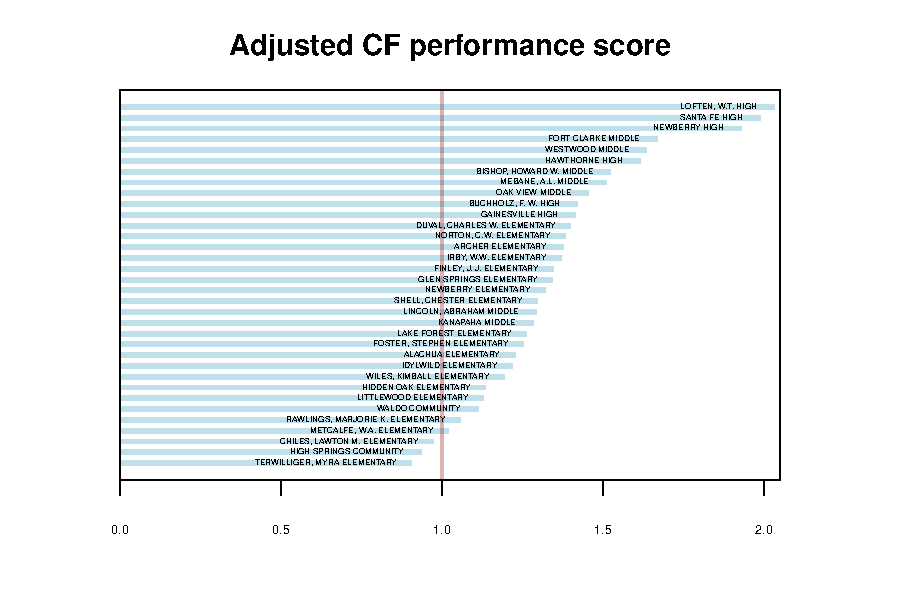
\includegraphics{targeting-016}


\begin{table}[H]
% latex table generated in R 3.1.1 by xtable 1.7-4 package
% Tue Dec 16 15:47:03 2014
\begin{table}[ht]
\centering
{\tiny
\begin{tabular}{lrrrr}
  \hline
SCHOOL & STUDENTS & EXPECTED & OBSERVED & SCORE \\ 
  \hline
LOFTEN, W.T. HIGH  & 198 & 59.04 & 120 & 2.03 \\ 
  SANTA FE HIGH  & 848 & 304.74 & 606 & 1.99 \\ 
  NEWBERRY HIGH  & 493 & 169.99 & 328 & 1.93 \\ 
  FORT CLARKE MIDDLE  & 804 & 420.63 & 702 & 1.67 \\ 
  WESTWOOD MIDDLE  & 928 & 458.36 & 750 & 1.64 \\ 
  HAWTHORNE HIGH  & 244 & 86.04 & 139 & 1.62 \\ 
  BISHOP, HOWARD W. MIDDLE  & 684 & 328.54 & 501 & 1.52 \\ 
  MEBANE, A.L. MIDDLE  & 365 & 181.45 & 274 & 1.51 \\ 
  OAK VIEW MIDDLE  & 671 & 382.80 & 557 & 1.46 \\ 
  BUCHHOLZ, F. W. HIGH  & 1970 & 722.44 & 1027 & 1.42 \\ 
  GAINESVILLE HIGH  & 1689 & 542.66 & 768 & 1.42 \\ 
  DUVAL, CHARLES W. ELEMENTARY & 284 & 159.94 & 224 & 1.40 \\ 
  NORTON, C.W. ELEMENTARY & 616 & 438.55 & 607 & 1.38 \\ 
  ARCHER ELEMENTARY  & 435 & 311.91 & 430 & 1.38 \\ 
  IRBY, W.W. ELEMENTARY & 375 & 268.50 & 368 & 1.37 \\ 
  FINLEY, J. J. ELEMENTARY & 523 & 373.41 & 503 & 1.35 \\ 
  GLEN SPRINGS ELEMENTARY & 455 & 333.10 & 448 & 1.34 \\ 
  NEWBERRY ELEMENTARY & 421 & 311.98 & 412 & 1.32 \\ 
  SHELL, CHESTER ELEMENTARY & 179 & 121.79 & 158 & 1.30 \\ 
  LINCOLN, ABRAHAM MIDDLE  & 643 & 313.31 & 405 & 1.29 \\ 
  KANAPAHA MIDDLE  & 907 & 473.77 & 608 & 1.28 \\ 
  LAKE FOREST ELEMENTARY & 282 & 159.85 & 202 & 1.26 \\ 
  FOSTER, STEPHEN ELEMENTARY & 460 & 318.54 & 399 & 1.25 \\ 
  ALACHUA ELEMENTARY & 347 & 240.42 & 295 & 1.23 \\ 
  IDYLWILD ELEMENTARY & 561 & 361.19 & 440 & 1.22 \\ 
  WILES, KIMBALL ELEMENTARY & 690 & 520.42 & 621 & 1.19 \\ 
  HIDDEN OAK ELEMENTARY & 653 & 496.25 & 564 & 1.14 \\ 
  LITTLEWOOD ELEMENTARY & 554 & 387.30 & 437 & 1.13 \\ 
  WALDO COMMUNITY  & 166 & 115.04 & 128 & 1.11 \\ 
  RAWLINGS, MARJORIE K. ELEMENTARY & 263 & 148.48 & 157 & 1.06 \\ 
  METCALFE, W.A. ELEMENTARY & 273 & 157.82 & 161 & 1.02 \\ 
  CHILES, LAWTON M. ELEMENTARY & 667 & 490.47 & 477 & 0.97 \\ 
  HIGH SPRINGS COMMUNITY  & 815 & 557.76 & 522 & 0.94 \\ 
  TERWILLIGER, MYRA ELEMENTARY & 275 & 176.43 & 160 & 0.91 \\ 
   \hline
\end{tabular}
}
\caption{Sociodemographic-adjusted consent form performance scores by school} 
\end{table}\end{table}

Of note in the above chart / table, high schools did much better than expected in 2013/14.  Also, the fact that only three schools achieved "lower than expected" consent form return rates is evidence of an overall trend towards higher consent form return.

\begin{center}
\end{center}


%%%%%%%%%%%%%%%%%%%%%%%%%%%%%%%%%%%%%%%%%%%%%%
% Immunization receptivity
%%%%%%%%%%%%%%%%%%%%%%%%%%%%%%%%%%%%%%%%%%%%%%
\newgeometry{margin = 2cm}
\begin{center}
\section*{2013-14 School evaluation: immunization receptivity}
\end{center}
\addcontentsline{toc}{section}{2013-14 School evaluation: immunization receptivity}
\begin{multicols}{2}
\setkeys{Gin}{width=0.51\textwidth}


\subsection*{Summary}
\addcontentsline{toc}{subsection}{Summary}

"Immunization receptivity" is the likelihood of saying "yes" on the consent form, given its return.  Though imperfect, it is a metric of how receptive / averse populations are to the concept of influenza immunization itself (independent of consent form return rate).  Hispanic students, students on free/reduced lunch, and students from rural schools appear to have the lowest levels of immunization receptivity.

\subsection*{Risk factors for immunization aversion}
\addcontentsline{toc}{subsection}{Risk factors for immunization aversion}


The following table provides adjusted odds ratios for saying "No" on a consent form, relative to the baseline group of white, non-free lunch, kindergarten-aged students. Here are two examples of how these odds ratios can be interpreted :\begin{enumerate}
\item "Holding constant other factors (grade and socioeconomic status), black students are only 1.12 more likely than white students to \textbf{not} consent to immunization."
\item "After adjustment for other factors (race and grade), students on free/reduced lunch are 1.48 times more likely to \textbf{not} consent to immunization than their non-free lunch counterparts."
\end{enumerate}




\begin{table}[H]
% latex table generated in R 3.1.1 by xtable 1.7-4 package
% Tue Dec 16 15:47:03 2014
\begin{table}[ht]
\centering
{\small
\begin{tabular}{lrr}
  \hline
Factor & Odds ratio & P-value \\ 
  \hline
Asian & 0.57 & 0.00 \\ 
  Hispanic & 1.53 & 0.00 \\ 
  Black & 1.14 & 0.00 \\ 
  Multiracial & 1.16 & 0.02 \\ 
  Native Amer. & 1.19 & 0.67 \\ 
  Grade 01 & 0.85 & 0.02 \\ 
  Grade 02 & 0.87 & 0.06 \\ 
  Grade 03 & 0.83 & 0.01 \\ 
  Grade 04 & 0.89 & 0.13 \\ 
  Grade 05 & 0.99 & 0.85 \\ 
  Grade 06 & 1.12 & 0.12 \\ 
  Grade 07 & 0.96 & 0.59 \\ 
  Grade 08 & 1.00 & 0.99 \\ 
  Grade 09 & 1.08 & 0.36 \\ 
  Grade 10 & 1.23 & 0.02 \\ 
  Grade 11 & 1.27 & 0.01 \\ 
  Grade 12 & 1.54 & 0.00 \\ 
  Free lunch & 1.45 & 0.00 \\ 
   \hline
\end{tabular}
}
\caption{Factors for immunization among CF returners} 
\end{table}\end{table}

\end{multicols}


\setkeys{Gin}{width=1\textwidth}

\begin{table}[H]
% latex table generated in R 3.1.1 by xtable 1.7-4 package
% Tue Dec 16 15:47:04 2014
\begin{table}[ht]
\centering
{\tiny
\begin{tabular}{lrrrr}
  \hline
SCHOOL & STUDENTS & EXPECTED & OBSERVED & SCORE \\ 
  \hline
LAKE FOREST ELEMENTARY & 202 & 106.11 & 129 & 1.22 \\ 
  LINCOLN, ABRAHAM MIDDLE  & 405 & 234.72 & 279 & 1.19 \\ 
  LOFTEN, W.T. HIGH  & 120 & 59.29 &  69 & 1.16 \\ 
  CHILES, LAWTON M. ELEMENTARY & 477 & 291.99 & 339 & 1.16 \\ 
  HIGH SPRINGS COMMUNITY  & 522 & 311.59 & 356 & 1.14 \\ 
  HIDDEN OAK ELEMENTARY & 564 & 352.28 & 397 & 1.13 \\ 
  WILES, KIMBALL ELEMENTARY & 621 & 382.66 & 428 & 1.12 \\ 
  DUVAL, CHARLES W. ELEMENTARY & 224 & 117.15 & 130 & 1.11 \\ 
  KANAPAHA MIDDLE  & 608 & 345.24 & 383 & 1.11 \\ 
  GAINESVILLE HIGH  & 768 & 404.93 & 440 & 1.09 \\ 
  FINLEY, J. J. ELEMENTARY & 503 & 293.21 & 317 & 1.08 \\ 
  METCALFE, W.A. ELEMENTARY & 161 & 85.52 &  92 & 1.08 \\ 
  BUCHHOLZ, F. W. HIGH  & 1027 & 558.21 & 600 & 1.07 \\ 
  NEWBERRY ELEMENTARY & 412 & 241.07 & 259 & 1.07 \\ 
  NEWBERRY HIGH  & 328 & 168.84 & 180 & 1.07 \\ 
  WESTWOOD MIDDLE  & 750 & 413.46 & 438 & 1.06 \\ 
  GLEN SPRINGS ELEMENTARY & 448 & 264.96 & 280 & 1.06 \\ 
  LITTLEWOOD ELEMENTARY & 437 & 251.18 & 259 & 1.03 \\ 
  TERWILLIGER, MYRA ELEMENTARY & 160 & 85.88 &  88 & 1.02 \\ 
  FOSTER, STEPHEN ELEMENTARY & 399 & 233.05 & 237 & 1.02 \\ 
  FORT CLARKE MIDDLE  & 702 & 397.95 & 398 & 1.00 \\ 
  BISHOP, HOWARD W. MIDDLE  & 501 & 278.03 & 277 & 1.00 \\ 
  SHELL, CHESTER ELEMENTARY & 158 & 87.53 &  87 & 0.99 \\ 
  ARCHER ELEMENTARY  & 430 & 250.61 & 249 & 0.99 \\ 
  OAK VIEW MIDDLE  & 557 & 316.40 & 309 & 0.98 \\ 
  ALACHUA ELEMENTARY & 295 & 168.93 & 164 & 0.97 \\ 
  NORTON, C.W. ELEMENTARY & 607 & 353.35 & 339 & 0.96 \\ 
  IDYLWILD ELEMENTARY & 440 & 239.56 & 229 & 0.96 \\ 
  IRBY, W.W. ELEMENTARY & 368 & 210.38 & 201 & 0.96 \\ 
  MEBANE, A.L. MIDDLE  & 274 & 147.76 & 141 & 0.95 \\ 
  RAWLINGS, MARJORIE K. ELEMENTARY & 157 & 81.99 &  78 & 0.95 \\ 
  WALDO COMMUNITY  & 128 & 71.75 &  63 & 0.88 \\ 
  HAWTHORNE HIGH  & 139 & 70.60 &  57 & 0.81 \\ 
  SANTA FE HIGH  & 606 & 318.15 & 230 & 0.72 \\ 
   \hline
\end{tabular}
}
\caption{Sociodemographic- and CFRR-adjusted immunization performance scores by school} 
\end{table}\end{table}


Of note in the above table, rural schools (Sante Fe, Hawthorne, Waldo, etc.) appear to have lower levels of immunization receptivity, relative to their urban and semi-urban counterparts.  Schools with a low immunization receptivity score can be expected to have lagging immunization rates, even if high consent form return rates were achieved.  Schools with the lowest immunization receptivity scores would likely benefit from educational interventions regarding facts and health benefits of flu immunization. It may advisable to target such interventions at families / parents. 



%%%%%%%%%%%%%%%%%%%%%%%%%%%%%%%%%%%%%%%%%%%%%%
% CONCLUSION
%%%%%%%%%%%%%%%%%%%%%%%%%%%%%%%%%%%%%%%%%%%%%%
\newgeometry{margin = 3cm}
\begin{center}
\section*{Conclusion}
\end{center}
\addcontentsline{toc}{section}{Conclusion}

\subsection*{Limitations and shortcomings}
This analysis has several limitations and shortcomings: \begin{enumerate}
\item Data were only complete through the 2013-14 school year.  \textbf{None} of the proceeding charts or calculations take into account the most recent flu season.
\item Consent form return, immunization, out-of-school immunization, and sociodemographic characteristics come from 4 different datasets (respectively EPI, Control Flu program data, Florida shots and ACPS).  Though great care was taken to combine data carefully, certain points were lost at every step of the way due to spelling inconsistencies and errors.  Though this report is likely \emph{representative} of true trends, it does not contain \emph{full} data.
\item Free/reduced lunch status is an imperfect proxy for socioeconomic status.
\item "Unobserved" variables (parental education, experience with health care system, etc.) likely explain a good portion of consent form return and immunization likelihood. "Grading" school performance based solely on the metrics in this report, therefore, could be problematic.  
\end{enumerate}

\subsection*{Current data analysis}
A similar evaluation of the 2014-15 flu season will be possible by March, thanks to (a) Paul Myers having secured access to Florida Shots data for this purpose and (b) Cuc Tran's team of EPI interns having digitized \emph{every} students' consent form return status.

\subsection*{Recommendations}
A fuller set of recommendations will be possible in light of the 2014-15 data analysis in March.  That said, the main take-aways from this report are: \begin{enumerate}
\item Statistical adjustment for confounding sociodemographic factors allows for a more "fair" evaluation of program performance by school.  The same principles can (and should) be applied in analysis of 2014-15 data, as well as analysis at a smaller scale (by classroom, etc.).  
\item "Expected" CF and immunization rates (by school, classroom or program team) can (and should) be calculated \emph{prior} to a flu season, allowing for the establishment of goals (ie, 110\% of expected).
\item After elementary school, increasing age is associated with a linear decline in the likelihood of consent form return.
\item Most of the variance in immunization rate can be explained by consent form return.  Differences between groups (race, socioeconomic status, age) would be greatly reduced if similar rates of consent form return were achieved.  Therefore, \textbf{consent form return} (and not immunization aversion) is the primary obstacle preventing higher immunization rates at most schools.
\item Non-Asian minorities are far less likely than their white counterparts to return a consent form.
\item Qualitative research may be needed to both (a) diagnose the reasons \emph{why} consent forms are not returned among certain groups and (b) assess potential culturally-relevant strategies for raising consent form return in these groups.  
\item A small number of schools have been identified (page 9) with higher than expected levels of vaccine aversion. Outreach / educational interventions targeting parents of children at these schools may be useful in raising immunization rates.
\end{enumerate}

%%%%%%%%%%%%%%%%%%%%%%%%%%%%%%%%%%%%%%%%%%%%%%
% DETAILS
%%%%%%%%%%%%%%%%%%%%%%%%%%%%%%%%%%%%%%%%%%%%%%
\newgeometry{margin = 3.5cm}
\begin{center}
\section*{Details}
\end{center}
\addcontentsline{toc}{section}{Details}

The analysis contained in this report was carried out for the purpose of improving Control Flu operations, and raising pediatric immunization rates in Alachua County.  The opinions, as well as in errors, are solely of the author, and do not represent or intend to represent DOH policy or practice. \\

The data used for this analysis are not available to the public.  That said, the statistical code and methods are accessible for review or replication: \\

\hyperref{https://github.com/joebrew/fdoh/tree/master/public/ab\_chd\_private}. \\


The data wrangling and analysis of this report was written in the R programming language (R version 3.1.1 (2014-07-10)), and the report production was programmed in Sweave and \LaTeX{} on a Windows i386-w64-mingw32 platform.\\



\end{document}
